\chapter{Quantum Complexity and Supremacy}\label{ch:complexity}
\begin{center}\small\textit{Where does quantum sit in the complexity zoo? From P to BQP to QMA, and the quest to prove advantage.}\end{center}

\section{Intuition: The Complexity Zoo}
Classical complexity sorts problems by resources: P (poly time), NP (poly proof verification), PSPACE, etc. Quantum complexity adds BQP (bounded-error quantum poly time) --- problems a quantum computer solves efficiently with error $\le1/3$ --- and QMA (quantum Merlin-Arthur) where the proof itself may be quantum. We know $\textsf{P}\subseteq\textsf{BQP}\subseteq\textsf{PSPACE}$ and $\textsf{NP}\subseteq\textsf{QMA}$, but whether BQP contains NP or vice versa is unknown. The placement matters: if $\textsf{NP}\subseteq\textsf{BQP}$, quantum breaks all NP cryptography; current belief is it does not, but BQP contains factoring and simulation tasks outside P.

\section{BQP and Friends}
\begin{definition}[BQP]
Language $L\in\textsf{BQP}$ if a uniform poly-size quantum circuit family decides $x\in L$ with $\Pr[\text{correct}]\ge2/3$ in $\mathrm{poly}(|x|)$ time, with bounded error.
\end{definition}
Error $1/3$ is arbitrary: repetition + majority amplifies to $1-2^{-\mathrm{poly}}$. BQP is the quantum analogue of BPP (bounded-error classical randomized poly time).

Key inclusions (strictness unknown except $\textsf{P}\neq\textsf{PSPACE}$):
\begin{equation}
\textsf{P}\subseteq\textsf{BPP}\subseteq\textsf{BQP}\subseteq\textsf{PP}\subseteq\textsf{PSPACE},\qquad
\textsf{NP}\subseteq\textsf{QMA},\ \textsf{BQP}\subseteq\textsf{QMA}.
\end{equation}

\begin{center}
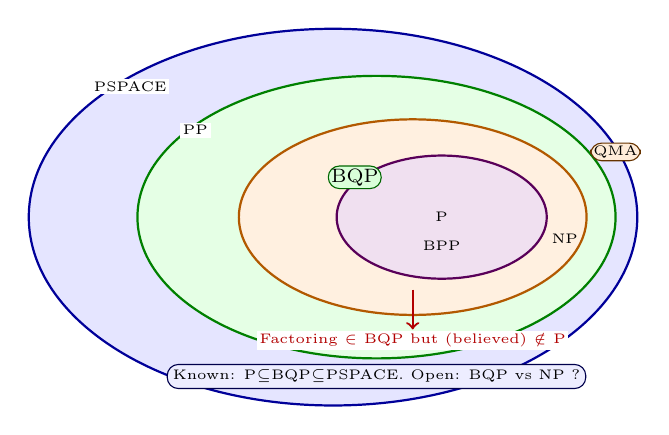
\begin{tikzpicture}[scale=0.92,font=\footnotesize]
  \fill[blue!10] (0,0) ellipse (4.2 and 2.6);
  \fill[green!10] (0.6,0) ellipse (3.3 and 1.95);
  \fill[orange!12] (1.1,0) ellipse (2.4 and 1.35);
  \fill[violet!12] (1.5,0) ellipse (1.45 and 0.85);
  \draw[thick, blue!60!black] (0,0) ellipse (4.2 and 2.6);
  \draw[thick, green!50!black] (0.6,0) ellipse (3.3 and 1.95);
  \draw[thick, orange!70!black] (1.1,0) ellipse (2.4 and 1.35);
  \draw[thick, violet!70!black] (1.5,0) ellipse (1.45 and 0.85);
  \node[font=\tiny, fill=white, inner sep=1pt] at (-2.8,1.8) {PSPACE};
  \node[font=\tiny, fill=white, inner sep=1pt] at (-1.9,1.2) {PP};
  \node[font=\scriptsize, fill=green!15, draw=green!40!black, rounded corners, inner sep=1pt] at (0.3,0.55) {BQP};
  \node[font=\tiny] at (1.5,0) {P};
  \node[font=\tiny] at (1.5,-0.4) {BPP};
  \node[font=\tiny, fill=orange!15, draw=orange!40!black, rounded corners, inner sep=1pt] at (3.9,0.9) {QMA};
  \node[font=\tiny] at (3.2,-0.3) {NP};
  \draw[->, thick, red!70!black] (1.1,-1.0)--(1.1,-1.55) node[below, font=\tiny, fill=white, inner sep=1pt] {Factoring $\in$ BQP but (believed) $\notin$ P};
  \node[font=\tiny, fill=blue!7, draw=blue!30!black, rounded corners, inner sep=2pt] at (0.6,-2.2) {Known: P$\subseteq$BQP$\subseteq$PSPACE. Open: BQP vs NP ?};
\end{tikzpicture}
\end{center}

\begin{definition}[QMA]
$L\in\textsf{QMA}$ if a poly-size quantum verifier $V$ exists such that: if $x\in L$, some poly-qubit witness $\lvert\psi\rangle$ makes $V$ accept with $\ge2/3$; if $x\notin L$, every $\lvert\psi\rangle$ makes $V$ accept with $\le1/3$.
\end{definition}
QMA-complete problem: local Hamiltonian --- estimate ground energy of a $k$-local quantum system (quantum analogue of SAT). This captures quantum chemistry difficulty.

\section{Quantum Supremacy / Advantage}
Supremacy: a quantum device performs a task no classical supercomputer can simulate in feasible time. Advantage: the task is also useful.

Google Sycamore (2019, 53 qubits) sampled random circuits in $200$\,s; classical estimate $10\,000$\,years (later reduced to days/weeks by better tensor-network simulation, but still exponential). Later photonic boson sampling (Jiuzhang) and IBM's utility experiments push the frontier.

\begin{center}
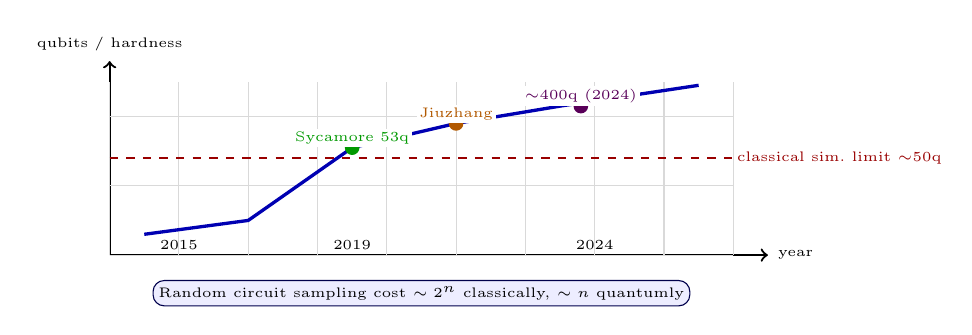
\begin{tikzpicture}[scale=0.88,font=\footnotesize]
  \draw[->, thick] (0,0)--(9.5,0) node[right, font=\tiny] {year};
  \draw[->, thick] (0,0)--(0,2.8) node[above, font=\tiny] {qubits / hardness};
  \draw[gray!30] (0,0) grid (9,2.5);
  % curve
  \draw[very thick, blue!70!black] (0.5,0.3)--(2.0,0.5)--(3.5,1.55)--(5.0,1.9)--(6.5,2.15)--(8.5,2.45);
  \fill[green!60!black] (3.5,1.55) circle (3pt) node[above, font=\tiny, fill=white, inner sep=1pt] {Sycamore 53q};
  \fill[orange!70!black] (5.0,1.9) circle (3pt) node[above, font=\tiny, fill=white, inner sep=1pt] {Jiuzhang};
  \fill[violet!70!black] (6.8,2.15) circle (3pt) node[above, font=\tiny, fill=white, inner sep=1pt] {$\sim$400q (2024)};
  \draw[dashed, red!60!black, thick] (0,1.4)--(9,1.4) node[right, font=\tiny, fill=white, inner sep=1pt] {classical sim.\ limit $\sim$50q};
  \node[font=\tiny] at (1.0,0.15) {2015};
  \node[font=\tiny] at (3.5,0.15) {2019};
  \node[font=\tiny] at (7.0,0.15) {2024};
  \node[fill=blue!7, draw=blue!30!black, rounded corners, inner sep=2pt, font=\tiny] at (4.5,-0.55) {Random circuit sampling cost $\sim2^n$ classically, $\sim n$ quantumly};
\end{tikzpicture}
\end{center}

Verification is the crux: how to check a supremacy experiment without classical simulation? Techniques include cross-entropy benchmarking (XEB), linear XEB, and interactive proofs. Complexity-theoretic evidence: if random circuit sampling were classically easy, the polynomial hierarchy would collapse (Aaronson--Arkhipov, Bremner--Jozsa--Shepherd).

\begin{center}
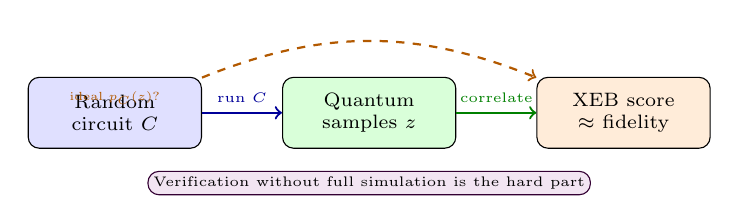
\begin{tikzpicture}[scale=0.85,font=\footnotesize]
  \node[draw, fill=blue!12, rounded corners, minimum width=2.2cm, minimum height=0.9cm, align=center, font=\scriptsize] (r) at (0,0) {Random\\circuit $C$};
  \node[draw, fill=green!15, rounded corners, minimum width=2.2cm, minimum height=0.9cm, align=center, font=\scriptsize] (q) at (3.8,0) {Quantum\\samples $z$};
  \node[draw, fill=orange!15, rounded corners, minimum width=2.2cm, minimum height=0.9cm, align=center, font=\scriptsize] (c) at (7.6,0) {XEB score\\$\approx$ fidelity};
  \draw[->, thick, blue!60!black] (r)--(q) node[midway, above, font=\tiny] {run $C$};
  \draw[->, thick, green!50!black] (q)--(c) node[midway, above, font=\tiny] {correlate};
  \draw[->, thick, orange!70!black, dashed] (r) to[bend left=22] (c) node[midway, above, font=\tiny] {ideal $p_C(z)$?};
  \node[font=\tiny, fill=violet!10, draw=violet!40!black, rounded corners, inner sep=2pt] at (3.8,-1.05) {Verification without full simulation is the hard part};
\end{tikzpicture}
\end{center}

\section{Oracular Separations}
We know relative to an oracle: $\textsf{BQP}\not\subseteq\textsf{PH}$ (Raz--Tal 2018, Forrelation problem) and oracles where $\textsf{BQP}\not\subseteq\textsf{NP}$ and $\textsf{NP}\not\subseteq\textsf{BQP}$. Hence quantum advantage is provable in black-box models, but unconditionally separating BQP from P or NP remains open --- as hard as classical $P\neq NP$.


\section{Beyond BQP: QMA and Local Hamiltonian}
QMA captures problems where a quantum witness helps. The $k$-local Hamiltonian problem: given $H=\sum_i H_i$ with each $H_i$ acting on $\le k$ qubits and numbers $a<b$ with $b-a\ge1/\mathrm{poly}(n)$, decide if ground energy $\lambda_{\min}\le a$ or $\ge b$. Kitaev showed this is QMA-complete for $k\ge2$, the quantum analogue of Cook--Levin's SAT completeness for NP. The proof gap $1/\mathrm{poly}$ is needed because quantum measurement is probabilistic.

No good quantum analogue of PH is settled; QPH and $\textsf{BQP/qpoly}$ explore advice. We also know $\textsf{BQP}\subseteq\textsf{PP}$: the acceptance probability of a quantum circuit is a \textsf{PP} sum, so quantum does not escape counting complexity.

\begin{example}[Simulating quantum is hard]
Exact simulation of $n$-qubit circuits costs $O(2^n)$ time/memory. Tensor networks help for shallow or low-entanglement circuits: matrix product states with bond $\chi$ cost $O(n\chi^3)$. Random circuits at depth $\sim\sqrt n$ maximize entanglement, defeating MPS --- hence their use for supremacy.
\end{example}

\section{Dequantization and Quantum Inspirations}
Ewin Tang's dequantization showed some QML speedups (recommendation systems) were not truly exponential once classical $\ell_2$-sampling assumptions matched quantum state assumptions. This sharpens the search for genuine advantage: problems with structure that resists $\ell_2$ dequantization, like quantum simulation and certain kernels, remain promising. Quantum-inspired classical algorithms are a healthy by-product of the quest.


\section{Interactive Proofs and Delegation}
QMA is one round; QIP (quantum interactive proofs) allows interaction and equals PSPACE (like classical IP=PSPACE). For delegation, Mahadev (2018) gave a protocol for a classical verifier to check a quantum computation assuming LWE hardness, using trapdoor claw-free functions. This bridges complexity theory and near-term verification of supremacy claims without trusting the device.


\section{Fine-Grained and Average-Case Hardness}
Worst-case hardness is not enough for cryptography; average-case matters. For random circuit sampling, Stockmeyer counting arguments plus conjectures about average-case \#P-hardness of approximating output probabilities support hardness. For BQP vs.\ PH, Raz--Tal's Forrelation problem gives an oracle separation with only $O(\log n)$ quantum queries vs.\ $\Omega(\sqrt n)$ classical --- unconditional in query model.


\section{Open Problems}
Is $\textsf{BPP}\neq\textsf{BQP}$ unconditionally? Is $\textsf{NP}\subseteq\textsf{BQP}$? Does $\textsf{BQP}\subseteq\textsf{PH}$? Each would be a major breakthrough. On the practical side, proving a superpolynomial advantage for a \emph{useful} problem (not oracular) with provable classical hardness remains open. Candidates include quantum simulation of strongly correlated materials and certain linear-algebra tasks under plausible assumptions.


\section{Proof Techniques}
Proving BQP lower bounds uses polynomial method (Beals et al.) and adversary method (Ambainis). Upper bounds use circuit constructions. For Forrelation, Raz--Tal combine Fourier analysis with pseudo-randomness to show classical decision trees need $\tilde\Omega(\sqrt N)$ queries while one quantum query suffices, separating BQP from PH relative to an oracle.



\begin{remark}[Why separations are hard]
Unconditional $\textsf{BQP}\neq\textsf{BPP}$ would imply $\textsf{P}\neq\textsf{PSPACE}$-level breakthroughs. Current gaps are conditional on assumptions (e.g., factoring not in BPP) or oracular. This mirrors classical $\textsf{P}\neq\textsf{NP}$ hardness and drives interest in fine-grained and average-case evidence.
\end{remark}

\section{Python: Complexity Scaling Demo}

\begin{lstlisting}[language=Python]
import math, random

def classical_random_circuit_cost(n, depth):
    """Rough ops to simulate n-qubit random circuit exactly: O(2^n)."""
    return 2**n * depth

def quantum_random_circuit_cost(n, depth):
    return n * depth  # linear in qubits

for n in [10, 20, 30, 50, 53]:
    c = classical_random_circuit_cost(n, 20)
    q = quantum_random_circuit_cost(n, 20)
    print(f"n={n:2d}  classical ~2^{n}={c:.1e} ops  quantum ~{q} ops  ratio {c/q:.1e}")

# Forrelation gap (Raz-Tal): quantum 1 query vs classical ~sqrt(N)
N = 1024
print(f"\nForrelation N={N}: quantum 1 query, classical ~{int(math.sqrt(N))} queries")
\end{lstlisting}

\begin{lstlisting}[language=Python]
# XEB fidelity estimation sketch
import numpy as np

def xeb_fidelity(samples, ideal_probs):
    """Linear XEB: F ~ N * mean(p_ideal(samples)) -1 ."""
    N = len(ideal_probs)
    mean_p = np.mean([ideal_probs[s] for s in samples])
    return N * mean_p - 1

# Ideal Porter-Thomas (random circuit) probs: exponential distribution
N = 1024
rng = np.random.default_rng(0)
ideal = rng.exponential(scale=1/N, size=N); ideal /= ideal.sum()
# Perfect quantum sampler
samples_perfect = rng.choice(N, size=5000, p=ideal)
# Noisy sampler (mix with uniform)
noisy_p = 0.7*ideal + 0.3*np.ones(N)/N
samples_noisy = rng.choice(N, size=5000, p=noisy_p)

print(f"XEB perfect ~{xeb_fidelity(samples_perfect, ideal):.3f} (expect 1.0)")
print(f"XEB noisy   ~{xeb_fidelity(samples_noisy, ideal):.3f} (expect ~0.7)")
print(f"Uniform XEB ~{xeb_fidelity(rng.choice(N,5000), ideal):.3f} (expect 0)")
\end{lstlisting}


\section{Unconditional vs.\ Conditional Gaps}
We have no unconditional proof that $\textsf{BPP}\neq\textsf{BQP}$ or $\textsf{P}\neq\textsf{PSPACE}$ implies $\textsf{BPP}\neq\textsf{BQP}$ open. Yet oracle separations are unconditional relative to that oracle. NREL? Also, $\textsf{BQP}\subseteq\textsf{PP}$ barrier suggests quantum advantage cannot be too strong: PP is in PSPACE, so exponential advantage beyond PP would place BQP outside PP, contradicting inclusion. The frontier is fine-grained: polynomial vs.\ super-polynomial separations.

Current research focuses on fine-grained advantage: e.g., $O(n^2)$ quantum vs.\ $\Omega(n^3)$ classical for linear systems (HHL) under sparsity and condition-number assumptions, or sample complexity gaps in learning theory where quantum PAC learning can be exponentially better for certain concept classes built from cryptography.


\begin{remark}[BQP in PP]
Acceptance probability $\Pr[\text{accept}]=\sum_z|\langle z|C|0\rangle|^2$ is a sum of exponentially many P-computable terms, a PP predicate: accept iff $\Pr>1/2$. Thus $\textsf{BQP}\subseteq\textsf{PP}\subseteq\textsf{PSPACE}$, bounding quantum advantage unconditionally.
\end{remark}

\begin{example}[Tensor-network simulation]
Depth $d$ 1-D circuits have entanglement $O(d)$, simulable via MPS with bond $\chi=2^{O(d)}$ and cost $O(n\chi^3)$. Random circuits at depth $\approx\sqrt n$ generate volume law $\chi\sim2^{n/2}$, defeating MPS. Hence supremacy circuits pick depth $\sim20$ for $n=53$.
\end{example}

\begin{remark}[Dequantization]
Tang's $\ell_2$-sampling algorithm matched quantum $O(\mathrm{poly}\log N)$ for recommendation under QRAM-like sampling assumptions. Lesson: exponential gaps need input-model qualification. Genuine advantage problems use structure like periodic or algebraic oracles that resist $\ell_2$ shortcuts.
\end{remark}

\section{Exercises}
\begin{exercise}
Show error $1/3$ in BQP can be amplified to $2^{-k}$ by $O(k)$ repetitions and majority vote. Why does this fail if error is $1/2$?
\end{exercise}
\begin{exercise}
Explain why factoring $\in$ BQP does not imply $\textsf{NP}\subseteq\textsf{BQP}$. What would $\textsf{NP}\subseteq\textsf{BQP}$ mean for lattice-based cryptography?
\end{exercise}
\begin{exercise}
State the local Hamiltonian problem and explain why it is QMA-complete (analogue of Cook--Levin). What parameter controls the promise gap?
\end{exercise}
\begin{exercise}
A 60-qubit random circuit has ideal output probabilities $\sim$Porter-Thomas. Estimate memory to store the full $2^{60}$ state vector in double precision. Why does this motivate XEB?
\end{exercise}
\begin{exercise}
Research the Sycamore vs.\ classical simulation debate: how did tensor-network improvements change the $10\,000$-year claim? What does this teach about supremacy definitions?
\end{exercise}
